\section{Linear Regression}
\framecard{\insertsection}
\subsection{Basic Concepts of Curve Fitting}

%
%

\subsection{Bayesian Curve Fitting}
\begin{frame}{\insertsubsection}
	\visible<1->{So, we'll start to look the regression with a statistical approach. To encourage you, let's take the sentence.}
	\visible<2>{\vspace{1.5em}
		\begin{block}{Sentence}
		\textit{If we could update the \textbf{\textcolor{red}{regression weights}} as we acquire some new values of the experiment?}
		\end{block}
   		     }
\end{frame}

\begin{frame}{\insertsubsection}
	\visible<1->{Let's take a look again at the Bayes Theorem}
	
	\visible<2->{
	\begin{block}{Bayes Theorem}{
			\begin{equation}\label{bayes_theorem}
				\visible<2->{ p(\mathbf{w}|\mathcal{D}) = \frac{p(\mathcal{D}| \mathbf{w}) \overbrace{ p(\mathbf{w})}^{\mathclap{\text{the \textit{a priori} probability}}}} { \underbrace{ p(\mathcal{D})}_{\mathclap{\text{the \textit{a priori} probability}}}} } 
			\end{equation}
			}
	\end{block}
	\visible<3->{So, if\textbf{ we have the probability} of the data, we'll could estimate the\textbf{ future weights}.}
	\visible<4>{\centering\textbf{\textcolor{red}{But, how?}}}
	}
\end{frame}

\begin{frame}{\insertsubsection}
	\visible<1->{Taking some steps back, let's re-visit the \textbf{Curve Fitting}. There, the strategy was minimize the error function.\vspace{1.5em} \\}
	\visible<2->{Now we'll try to view the same problem with a \textit{probabilistic perspective}. We're trying to make predictions for the target value $\boldsymbol{t}$ given some new values of $x$.\vspace{1.5em} \\}
	\visible<3->{A good ideia is to express our target values $\boldsymbol{t}$ in terms of \textbf{gaussians distributions} with the mean equals to $y(x,\mathbf{w})$.}
\end{frame}

\begin{frame}{\insertsubsection}
	\begin{figure}
		\label{schematic-gaussian-distribution}
		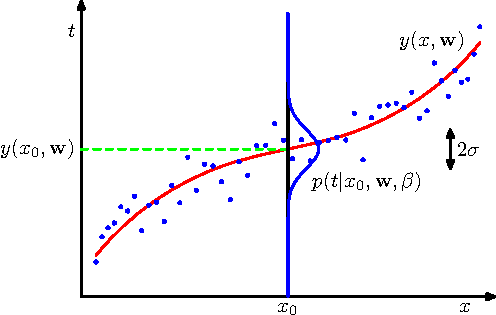
\includegraphics[totalheight=0.6\textheight]{Figure1c16.pdf}
		\caption{Schematic of the polynomial function $y(x,\mathbf{w})$ and the gaussian distribution $p$.}

	\end{figure}
\end{frame}


\begin{frame}{Title}
  $
    blah =
    \only<1>{blah}
    \only<2>{result}
    \visible<1>{%
      =
      \begin{cases}
          blah \\ 
          blah
        \end{cases}
      }
    $
\end{frame}